For each year, we found the 'hottest' high and the 'coolest' low. These values were plotted side-by-side, with the y-axis showing temperature and the x-axis showing the years 2000 - 2021. 2022 was excluded in both the 'highest highs' and 'lowest lows' graphs, since the year's temperatures are not completed yet. The highest recorded temperatures are shown below. 2011 had the hottest year on record, reaching a temperature of 114 degrees Farenheit on August 3rd, 2011. This value was confirmed with an article from the Arkansas Democrat Gazette talking about the intense heat on August 4th, 2011 \cite{historic_high}.

\begin{figure}[h!]
\centering
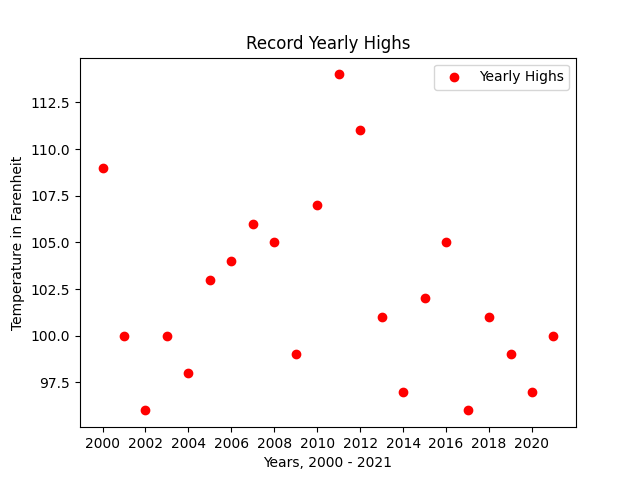
\includegraphics[scale=0.8]{Highs.png}
\label{Figure 1: Record Highs}
\caption{Figure 1: Record Highs, data from NOWData.}
\end{figure}
\FloatBarrier

\begin{figure}[h!]
\centering
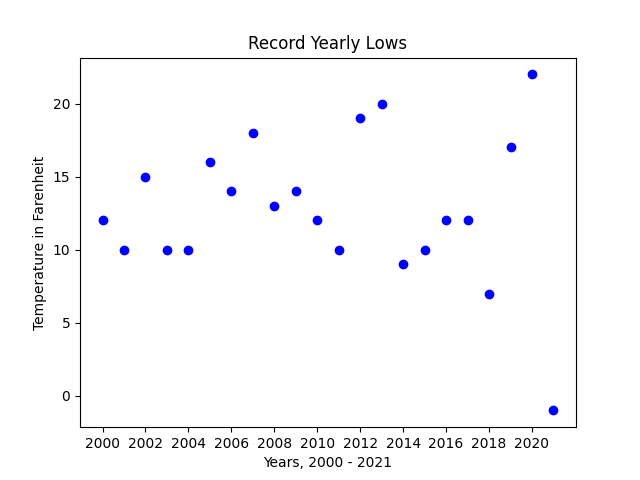
\includegraphics[scale=0.8]{Lows.png}
\label{Figure 2: Record Lows}
\caption{Figure 2: Record Lows, data from NOWData.}
\end{figure}
\FloatBarrier

Figure 2 shows the years' lowest lows, with the record being recently on Febuary 16th, 2021, at -1 degrees Farenheit.
